\documentclass[aspectratio=169,10pt]{beamer}
\usetheme{Boadilla}
\usecolortheme{seahorse}
\usepackage{graphicx}
\usepackage{booktabs}
\usepackage{tikz}
\usetikzlibrary{arrows.meta,positioning}
\setbeamertemplate{navigation symbols}{}
\setbeamertemplate{footline}[frame number]
\setbeamercolor{structure}{fg=teal!65!black}
\setbeamercolor{alerted text}{fg=red!70!black}
\title[JalRakshak]{JalRakshak: Smart Water Purification and Quality Monitoring}
\subtitle{A low-cost IoT and machine-learning software prototype for rural and mining-affected Jharkhand}
\author[Nischal Singhania and Animesh Giri]{Nischal Kumar Singhania \and Animesh Giri}
\institute{B.Tech Computer Science and Engineering (CCVT) · Third Year}
\date{Research project presentation · 2026}
\begin{document}

\begin{frame}
  \titlepage
  \vspace{-0.6em}
  \begin{center}
    \footnotesize Software prototype: implemented and locally tested. Sensor hardware and laboratory validation are separate pending stages.
  \end{center}
\end{frame}

\begin{frame}{Problem and research objective}
\begin{columns}[T,onlytextwidth]
  \column{0.56\textwidth}
  \begin{block}{Why this matters}
    \begin{itemize}
      \item Groundwater quality can vary across rural and mining-affected sites.
      \item A purifier indicator or single TDS meter does not provide parameter history or explain changing conditions.
      \item Communities need a low-cost way to observe raw and treated water trends and receive understandable alerts.
    \end{itemize}
  \end{block}
  \column{0.41\textwidth}
  \begin{block}{Research questions}
    Can one software workflow combine parameter monitoring, threshold alerts, short-term forecasts and anomaly screening? How does the workflow behave under noise, missing readings and drift?
  \end{block}
  \begin{alertblock}{Safety boundary}
    pH, turbidity, TDS and temperature do not establish pathogen or heavy-metal safety. Laboratory tests are essential.
  \end{alertblock}
\end{columns}
\vfill
{\tiny Limits: IS 10500:2012 (Second Revision, as amended); WHO Guidelines for Drinking-water Quality, 2026 edition.}
\end{frame}

\begin{frame}{Implemented software architecture}
\begin{block}{Two distinct input paths}
\centering
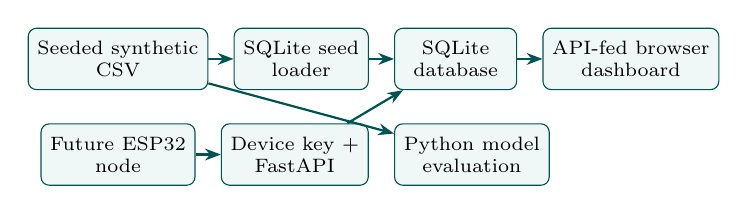
\begin{tikzpicture}[node distance=0.32cm,
  n/.style={draw=teal!65!black,fill=teal!6,rounded corners=3pt,align=center,minimum height=0.78cm,minimum width=1.55cm,font=\scriptsize},
  a/.style={-{Stealth[length=2mm]},thick,teal!65!black}]
  \node[n] (csv) {Seeded synthetic\\CSV};
  \node[n,right=of csv] (seed) {SQLite seed\\loader};
  \node[n,right=of seed] (db) {SQLite\\database};
  \node[n,right=of db] (ui) {API-fed browser\\dashboard};
  \node[n,below=0.42cm of csv] (esp) {Future ESP32\\node};
  \node[n,right=of esp] (api) {Device key +\\FastAPI};
  \node[n,right=of api] (ml) {Python model\\evaluation};
  \draw[a] (csv)--(seed); \draw[a] (seed)--(db); \draw[a] (db)--(ui);
  \draw[a] (esp)--(api); \draw[a] (api)--(db); \draw[a] (csv)--(ml);
\end{tikzpicture}
\end{block}
\begin{columns}[T,onlytextwidth]
  \column{0.48\textwidth}
  \begin{block}{Software delivered}
    Authenticated device ingestion; range and timestamp validation; duplicate prevention; SQLite persistence; API-backed dashboard; reproducible CSV experiments.
  \end{block}
  \column{0.49\textwidth}
  \begin{block}{Treatment design}
    Sediment and carbon pre-treatment; membrane selected from water chemistry; UV only with validated dose and flow. Remaining-life indicators are simulated estimates.
  \end{block}
\end{columns}
\vspace{0.15em}
{\tiny The CSV is loaded by a seed script and read directly by Python experiments. The physical ESP32 input path is supplied as a firmware template only.}
\end{frame}

\begin{frame}{Reproducible experiment and measured outputs}
\begin{columns}[T,onlytextwidth]
  \column{0.33\textwidth}
  \begin{block}{Dataset}
    \begin{itemize}
      \item 504 synthetic hourly records
      \item 3 illustrative devices
      \item 168 hours/device
      \item 70/30 chronological split
      \item 10 sensitivity conditions plus baseline
    \end{itemize}
  \end{block}
  \column{0.64\textwidth}
  \begin{block}{One-hour forecast error (lower is better)}
    \centering\scriptsize
    \begin{tabular}{lrrrr}
      \toprule
      & \multicolumn{2}{c}{TDS} & \multicolumn{2}{c}{Turbidity}\\
      \cmidrule(lr){2-3}\cmidrule(lr){4-5}
      Model & MAE & RMSE & MAE & RMSE\\
      \midrule
      Persistence & \textbf{9.34} & \textbf{20.39} & \textbf{0.080} & \textbf{0.247}\\
      Linear regression & 79.02 & 147.31 & 0.278 & 0.516\\
      Random forest & 74.05 & 143.94 & 0.093 & 0.332\\
      \bottomrule
    \end{tabular}
  \end{block}
  \begin{block}{Isolation Forest}
    Precision 0.796 · Recall 0.582 · F1 0.672 (153 held-out rows)
  \end{block}
\end{columns}
{\tiny Synthetic data only. The persistence model outperformed the two regressors on these one-hour targets.}
\end{frame}

\begin{frame}{Verification, outcome and remaining boundary}
\begin{columns}[T,onlytextwidth]
  \column{0.53\textwidth}
  \begin{block}{Locally verified software}
    \begin{itemize}
      \item 17 automated tests passed.
      \item 504-row seed import; second import adds no duplicates.
      \item Device authentication, validation, persistence and alert state updates tested.
      \item Forecast, anomaly and 10-condition robustness outputs reproducible.
      \end{itemize}
  \end{block}
  \begin{block}{Evidence-based finding}
    More complex regressors did not beat persistence on the generated series. Missingness and noise changed the anomaly score; results remain simulator-specific.
  \end{block}
  \column{0.44\textwidth}
  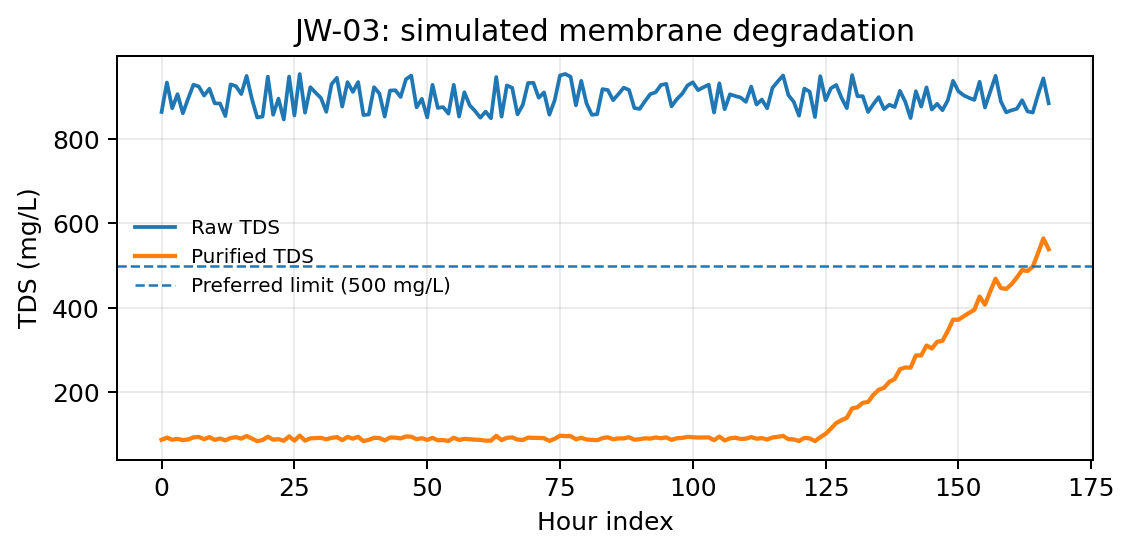
\includegraphics[width=\linewidth,height=3.0cm,keepaspectratio]{figures/jw03_tds_series.png}
  \vspace{0.2em}
  {\tiny Example synthetic JW-03 series.}
  \begin{alertblock}{Not yet field validated}
    ESP32 sketch is an uncompiled integration template. Physical calibration, treated-water lab analysis, UV dose/flow checks and supervised field trials remain required before any safety claim.
  \end{alertblock}
\end{columns}
\end{frame}
\end{document}
